\chapter{lnverse ray mapping for systems with Fresnel reflection}
\label{chap:fresnel}
In this chapter we present the inverse ray mapping method for systems formed optical lines for which Fresnel reflection can occur. The system is located into two different materials. Every time that a ray hits an optical line, a part of it is reflected and a part is refracted. 
%The amount of light that is reflected and refracted is given by the reflectance and transmittance which are related to Fresnel coefficients (see ). 
Hence, a ray emitted from the source generates two rays after interactions with the optical lines (the reflected ray and the transmitted one) each of them has the percentage of the original power given by the reflectance $\mathcal{R}$ and the transmittance $\mathcal{T}$ obtained from Fresnel equations (see Section \ref{sec:fresnel}).
At the next intersection of the two rays with a line, each incident ray is split
again. This process is called ray splitting. The ray emitted from the source is called the parent rays. Once the ray hits a line one of the two rays keeps the parent status while the other one is called child ray. The convention is to assign the parent status to the ray with the most power.
This results tracing a rapidly increasing number of rays, including those with a very little power (at every interaction the power of the ray decreases). 
Many different paths can occur and the number of paths is determined considering all the possible combinations that a ray can have. The number of possibilities increases with the number of optical lines that form the systems. For example, for a system formed by a source, a Fresnel line and a target, two possibilities can occur since a ray emitted from the source can either refract reaching the target or reflect going back to the source. Note that no scattering phenomena are considering in this thesis. If a system is formed by a source, two Fresnel lines and a target much more paths are possible since the ray can reflect forward and backward between the two optical lines before arriving either at the target or at the source again. For systems where multiple reflections can occur the number of paths can increases dramatically. 
Ray splitting is a powerful method to calculate \textit{all} physical paths but it generates more and more rays many of which are not significant for computing the target intensity. This makes ray splitting methods time consuming. 
\\ \indent
MC and QMC ray tracing consider a single ray every time that it hits an optical line. The transmittance $\mathcal{T}$ and reflectance $\mathcal{R}$ are determined at every intersection between the ray and the line. Next, a randomly generated number between $0$ and $1$ establishes which path the rays will continue to follow. Usually the assumption that when $\mathcal{R}$ is greater than the random number, the reflected ray is considered, otherwise the transmitted one is taken into account. Therefore, for each ray traced a unique path is possible and the number of rays emitted from the source corresponds to the total number of rays traced, \cite{koshel2012illumination}. Compared to methods that consider all possible paths of each ray, MC and QMC are easy to implement and the computational time required to achieve a good accuracy is reduced. However it has some disadvantages. First, part of the energy is lost, therefore the luminance at the target will be always less than the luminance at the source of the system. To achieve a very accurate luminance or intensity distribution at the target, more rays need to be traced such that more paths will be considered.
Second, it can beneficial in proper modeling of an optical system to consider ray splitting.
% Explain better 
\\ \indent 
To improve the exiting methods we here apply the numerical inverse ray mapping explained in the previous chapters to systems formed by Fresnel lines. For every incident ray we take into account of both the reflected and the refracted ray. Therefore, for a given position and direction of a ray emitted by the source at least two possible paths are allowed. Therefore, it can happen that more than one path from the source to the target is permitted for the same initial coordinates of a ray. A point in source PS ray in source PS can be associated to two or more points in target PS. Therefore, considering Fresnel reflections, the regions in target PS formed by the rays that follow the same path overlap. This would not make the inverse ray mapping suitable for this systems.
\\ \indent To overcome this issue we modify the inverse ray mapping applied to systems with only refractive lines by considering the physical paths one by one. To include Fresnel reflection, every time that the inverse ray tracing is applied, we consider either the reflected of the refracted ray depending on the path to which we want to determine the boundary. This allows determining the boundaries of the corresponding region in target PS. Furthermore, the power of every ray at each intersection with a line is calculated. Hence, once the rays on the boundaries are determined, their corresponding power at the target is also calculated. Note that the luminance at the target cannot be constant along a given direction and it depends on both the position and the direction. To determine the luminance related to the rays that follow a certain path, an interpolation between the rays on the corresponding boundary in PS is done along every direction. The procedure is repeated for every path (or for all the paths needed to obtain a good accuracy). The partial luminance related to every path is computed.
The total luminance is given by the sum of all the partial luminance calculated.
Finally, the intensity is given an integration of the luminance along all the possible positions.
\\ \indent
The method is presented in detail in the next section for a simple system where Fresnel reflection plays a role.
\section{Inverse ray mapping for a Fresnel lens}
In this section we present the numerical  inverse ray mapping for a simple optical system formed by the source, the target and a Fresnel lens.
% Why is important
First we describe the geometry of the system, then we explain the method for this system.
\subsection{The geometry of the system}
Let us consider the optical system depicted in Figure \ref{fig:lens}. 
% Geometry of the system
\begin{figure}[t]
  \begin{center}
  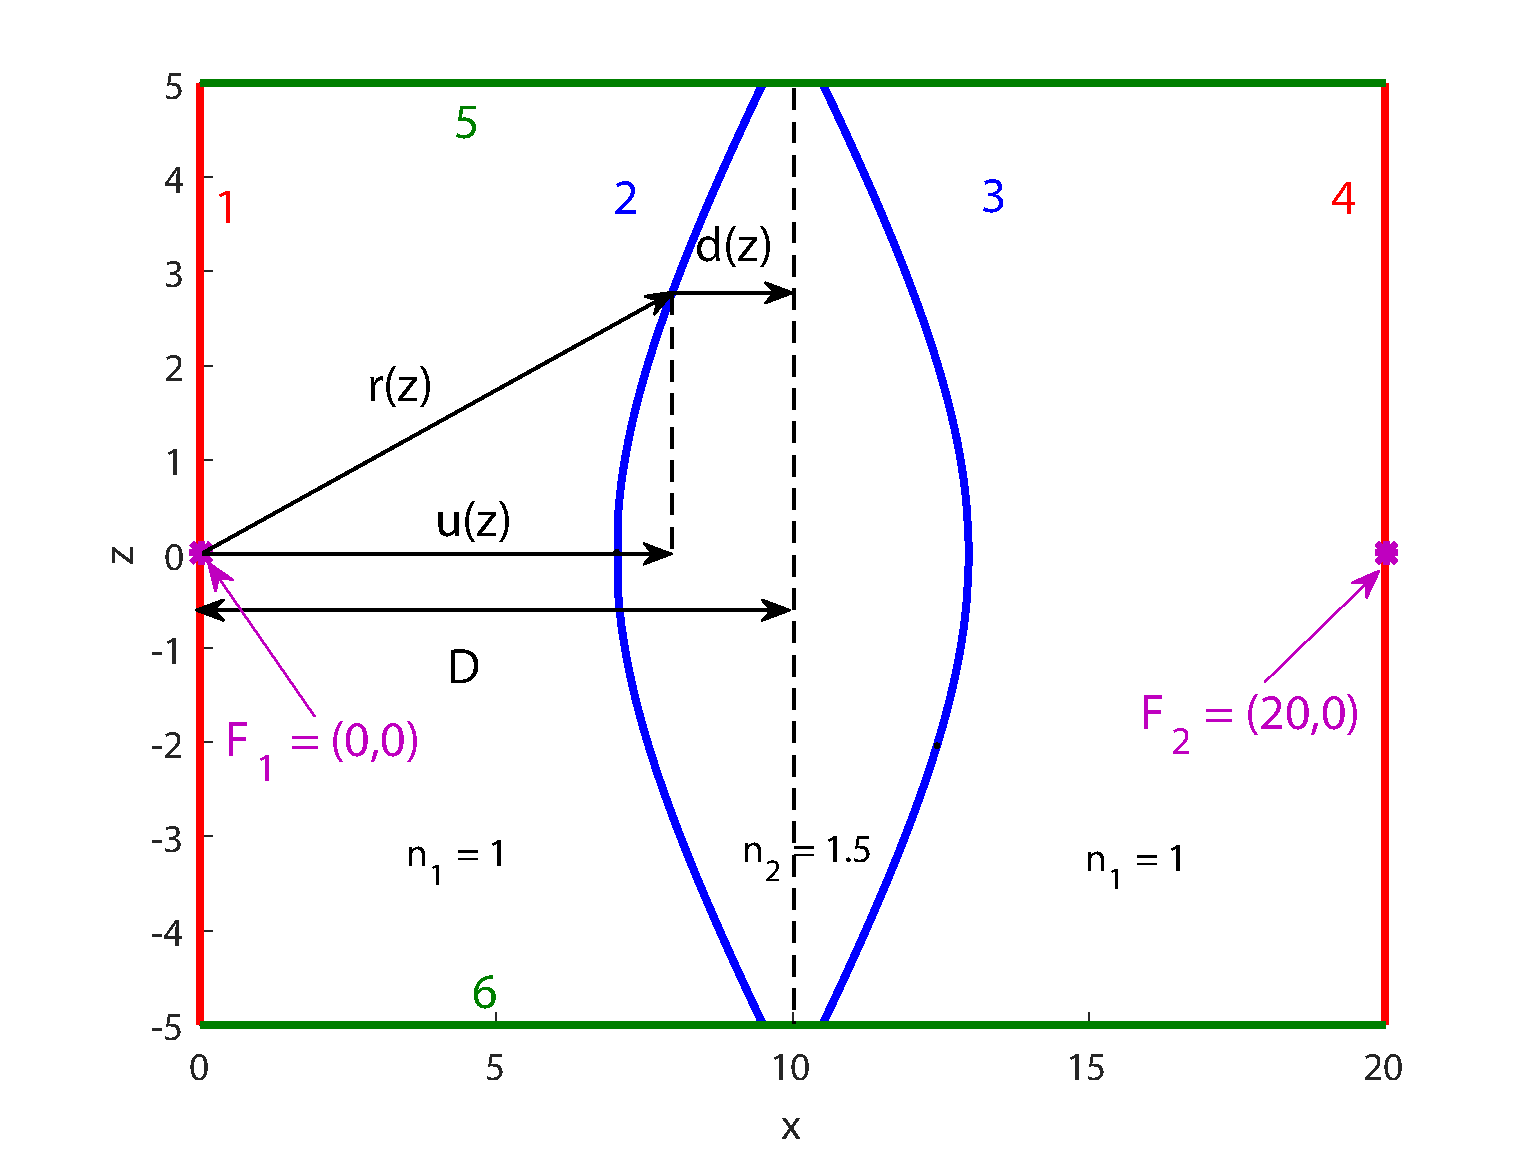
\includegraphics[width=0.6\textwidth]{lens}
  \end{center}
  \caption{\textbf{A Fresnel lens}
The source (line $1$) and the target (line $4$) are located in air ($\n = 1$), the material between lines $2$ and $3$ has index of refraction $\n=1.5$. 
Two reflectors (lines $5$ and $6$) are located at the top and the bottom of the lens to detect light exiting from the system.}
\label{fig:lens}
 \end{figure}
It is formed by the source (line $1$), a lens formed by two optical lines (line $2$ and $3$), the target (line $4$) and two detectors (line $5$ and $6$) at the top and the bottom of the system. The source \point{S} is a vertical line segment located at $\variabile{x}=0$ and with 
$\variabile{z}\in[-\variabile{h}, \variabile{h}]$ where $\variabile{h}=5$. The target \point{T} is a line segment of the same length of the source \point{S}, parallel to \point{S} and located at a distance $\variabile{x}=\variabile{a}$ from \point{S} with $\variabile{a} = 20$. The lens is formed by two refractive lines (simple lens), and it is convex as it is thicker at its middle point than at its edges.
The lines $2$ and $3$ that form the lens are symmetric to each other with respect to the axis $\variabile{x}=10$. The optical axis is the line $\variabile{z}=0$. $D=10$, $\variabile{h}=5$, $\textrm{d}(5)=0.5$.
% Citation
\begin{figure}[t]
  \begin{center}
  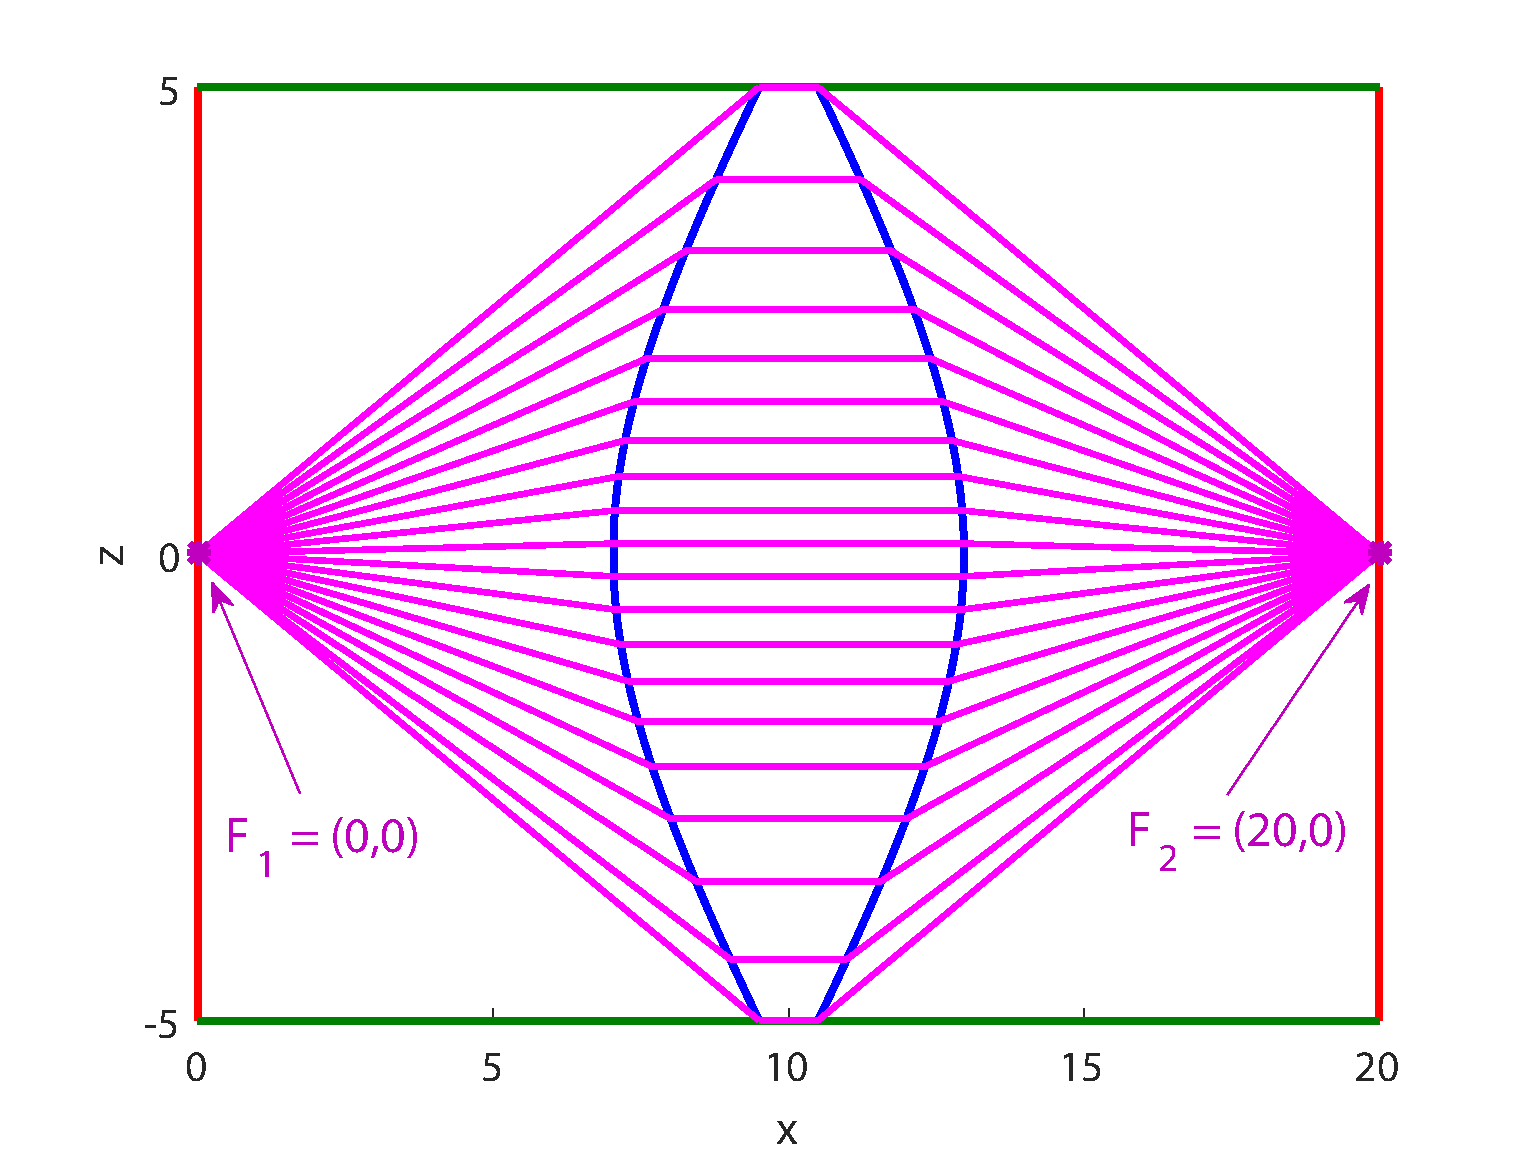
\includegraphics[width=0.6\textwidth]{lens_rays}
  \end{center}
  \caption{\textbf{A Fresnel lens.} 
All the rays exiting from $\point{F}_1$ arrive at $\point{F}_2$.}
\label{fig:real-lens}
 \end{figure}
\\ \indent To derive the equations of the curved lines we impose that the optical path length is constant. In the following we explain how equation for the left lens (line $2$) is obtained. We indicating with $\variabile{d}(\variabile{z})$ half of the lens thickness at high $\variabile{z}$, with $\vect{r}(\variabile{z})$ the parametrization of the ray emitted from $\point{F}_1$ and that reaches line $2$ at high $\variabile{z}$, $u(\variabile{z})$ is the projection of $\vect{r}(\variabile{z})$ on the optical axis and $D=10$ is the distance between the $\point{F}_1$ and the axis $\variabile{x}=10$.
The following relations hold:
\begin{equation}\label{eq:variables_lens}
\begin{aligned}
\vect{r}^{2\,}(\variabile{z}) &= (u(\variabile{z}))^2+\variabile{z}^{\,2},\\
u(\variabile{z}) &= (D-\variabile{d}(\variabile{z}))^2, 
\end{aligned}
\end{equation}
The optical path length is given by:
\begin{equation}\label{eq:path_length}
|\vect{r}(\variabile{z})|+n_2|\variabile{d}(\variabile{z})|=\tilde{C},
\end{equation}  
where $\tilde{C}$ is a constant greater than $0$. Substituting Equations (\ref{eq:variables_lens}) in the previous equation,
we obtain for every $\variabile{z}\in[-\variabile{h}, \variabile{h}]$ the expression for line $2$ given by:
\begin{equation}
Au(\variabile{z})^2+B(\variabile{z})+C+\variabile{z}^2 = 0
\end{equation}
where 
\begin{equation}
\begin{aligned}
A & = (1-\n_2^2), \\
B & = 2\n_2(\n_2 D-\tilde{C}), \\
C & = -\tilde{C}^2+2\n_2 D\tilde{C}-\n_2^2D^2. \\
\end{aligned}
\end{equation}
The right lens is given by a reflection with respect to the axis $\variabile{x}=0$ and a translation $(\variabile{x}, \variabile{z})\rightarrow (\variabile{x}+20, \variabile{z})$.
\\ \indent The lens constructed in this way has the property that every ray that hits each curved line is bent towards the optical axis. The rays passing through it connect the conjugate points $\point{F}_1 = (0, 0)$ and $\point{F}_2= (\variabile{a}, 0)$ which are the focal points of line $2$ and $3$ respectively (see Figure \ref{fig:real-lens}). Therefore, all the rays diverging from $\point{F}_1$ converge to $\point{F}_2$. In the next section we explain how to apply the numerical inverse ray mapping to this system.
\subsection{The explanation of the method}
Our goal is to show that, using the full inverse ray mapping, we can detect \textit{all} the possible paths limiting the number of rays traced.
First, let us analyze the inverse ray tracing process for the system in Figure \ref{fig:lens} introduced in the previous section. Every ray is emitted from the source $\point{S}$ with an angle $\myangle_1\in[-\frac{\pi}{2}, \frac{\pi}{2}]$, that is with a direction $\variabile{p}_1\in[-1,1]$. Every time that a ray hits a Fresnel lens, i.e. either line $2$ or $3$, the ray is split in two rays, the reflected ray and the refracted one. The reflectance $\mathcal{R}$ and the transmittance $\mathcal{T}$ are calculated. The reflected ray will continue to propagate within the system with the percentage of power given by $\mathcal{R}$. Similarly the transmitted ray will travel inside the system with the power obtained by $\mathcal{T}$. The trajectory of each ray is stopped either when it arrives at the target \point{T} or when it reaches again the source \point{S}. This leads to many different paths for a single ray with a given initial position and direction. Note that at every interaction with a Fresnel line the ray loses some energy due to the fact that it is divided into two more rays.\\ \indent
%To avoid that rays with a small power are traced through the system some ray tracing methods have been developed such that either the reflected or the refracted part of each ray is considered at every intersection with a Fresnel line. Therefore all the number of ray emitted from the source equals the number of total rays traced as no splitting is considered.  
MC and QMC methods are examples of such processes. The ray that has to be taken into account is decided randomly. This results tracing less rays as those with many reflections inside the system are discarded. 
\\ \indent 
%To detect the rays with more reflections using either MC or QMC ray tracing, more rays are needed. The number of paths possible are much more, potentially infinity paths.  
\\ \indent
We start considering the target PS of the system in Figure \ref{fig:lens}. Since, for the system in Figure \ref{fig:lens} the source and the target are vertical lines (the $\variabile{x}$ coordinates are fixed while varying the $\variabile{z}$ coordinates), the PS coordinates are $(\variabile{q}, \variabile{p})$, where  $\variabile{p}$ is the ray direction coordinate defined as for the previous systems while $\variabile{q}$ is the $\variabile{z}$ coordinate of the $\variabile{x}$ coordinate. To have an idea of the rays distribution at the target we represent the target coordinates on PS of $10^4$ rays traced using QMC ray tracing. 
Running QMC ray tracing for the lens in Figure \ref{fig:lens} with $10^4$ rays and storing the corresponding paths, the following three paths are found:
\begin{equation}\label{eq:paths_fresnel}
\begin{aligned}
\Pi_1 & = (1,2,3,4),\\
\Pi_2 & = (1,2,3,2,3,4), \\
\Pi_3 & = (1,2,3,2,3,2,3,4).
\end{aligned}
\end{equation}
In Figure \ref{fig:target_PS_lens} we provide the target PS of the Fresnel lens where we depicted with the same color the rays that follow the same path. The rays in magenta are rays that follow path $\Pi_1$, the cyan rays have two reflections before reaching the target following path $\Pi_2$, the black rays have three reflections inside the lens, these rays follow path $\Pi_3$ (see Equation (\ref{eq:paths_fresnel})).
\begin{figure}[t]
  \begin{center}
  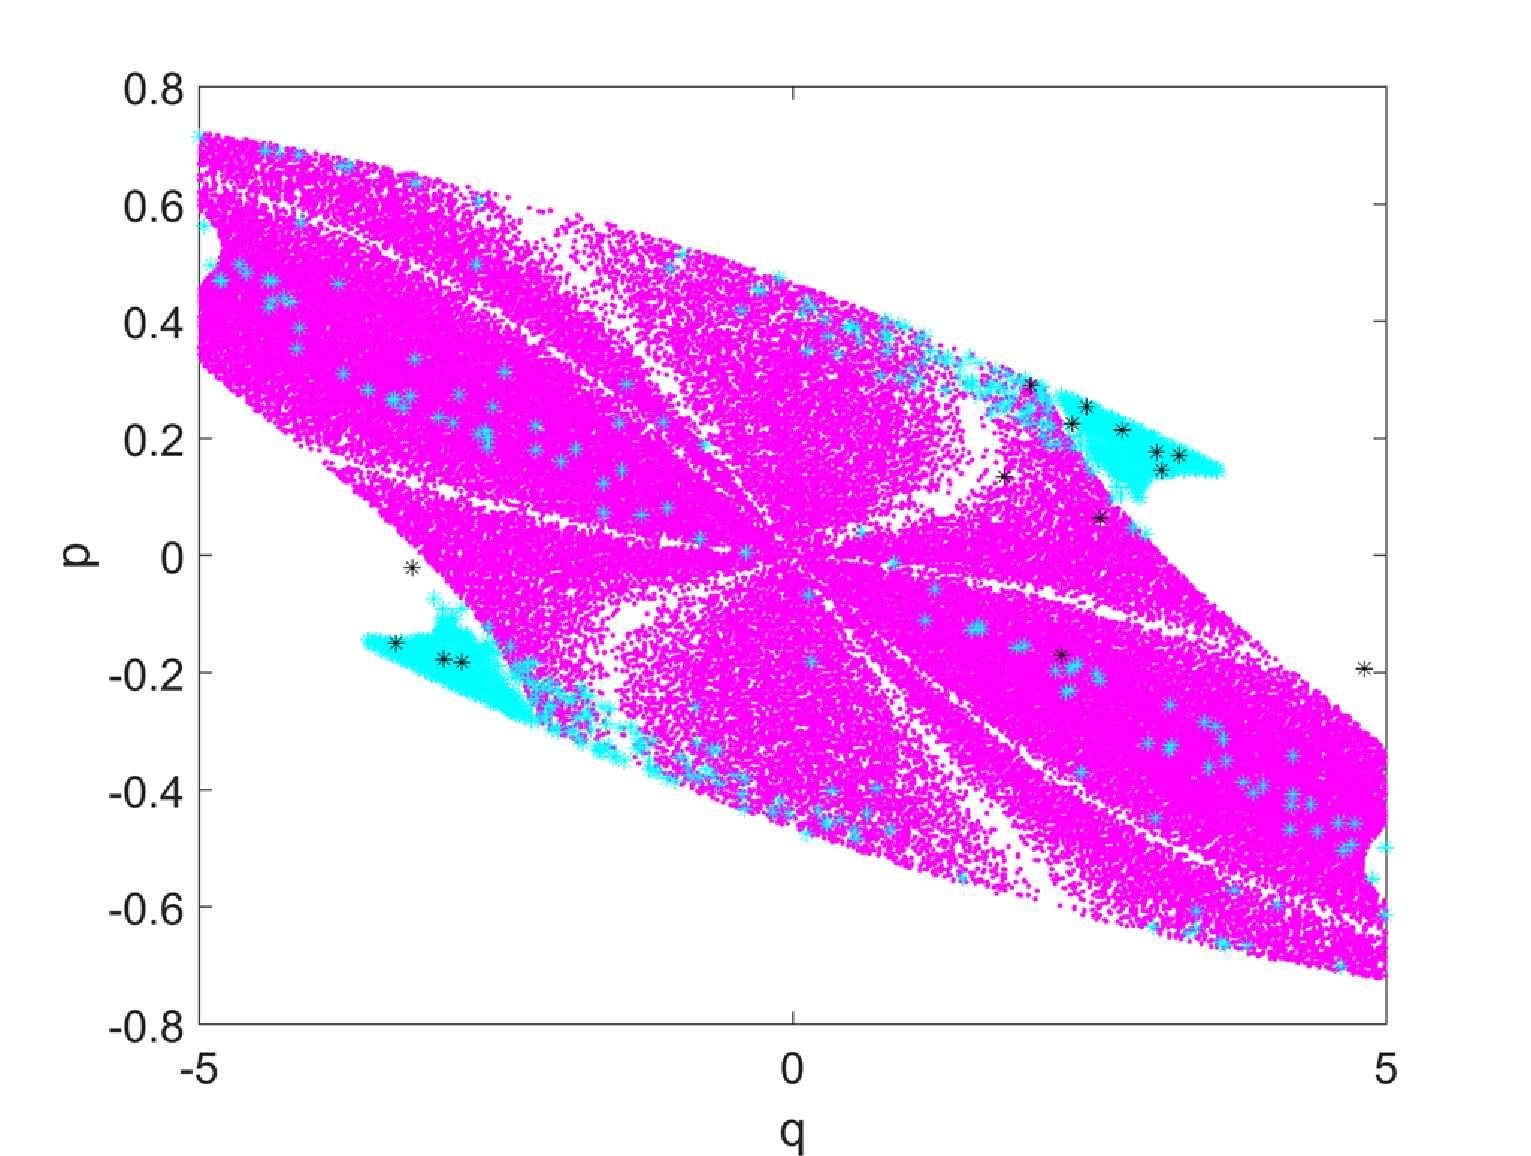
\includegraphics[width=0.6\textwidth]{target_lens}
  \end{center}
  \caption{\textbf{Target PS of the Fresnel lens}
The magenta rays follow path $\Pi_1$, the cyan rays follow path $\Pi_2$ and the black rays follow path $\Pi_3$.}
\label{fig:target_PS_lens}
 \end{figure}
We observe that the rays with more reflections have a less frequency inside the system. Furthermore, some areas inside the region \set{R}{}{}$(\Pi_1)$ are not covered by any ray (white parts). Therefore, rays that leave two close position coordinates at the source with a close direction coordinates can follow different paths during their propagation. This can be due to either TIR or a different choice of rays (reflected or refracted) at the intersections with Fresnel lines. In the first case, the rays will be located outside the region \set{R}{}{}$(\Pi_1)$, otherwise they can reach the interior of \set{R}{}{}$(\Pi_1)$. The latter case implies that, given two different paths $\Pi_{\variabile{i}}$ and $\Pi_{\variabile{j}}$ with $\variabile{i}\neq\variabile{j}$, the corresponding regions \set{R}{}{}$(\Pi_{\variabile{i}})$ and \set{R}{}{}$(\Pi_{\variabile{j}})$ can overlap in target PS. Thus:
\begin{equation}
\bigcap_{\Pi}\mbox{\set{R}{}{}}(\Pi)\neq \emptyset
\end{equation}
where the intersection is over all the possible paths. 
% Say that simply applying bisection and ray tracing is not enough
Because of this, we need to slightly modify the full inverse ray mapping explained in the previous chapter to detect all the possible paths. \\ \indent
The idea is to apply the bisection method combined with the inverse ray tracing to the entire PS for every single path $\Pi$ separately. All the possible paths from the target to the source can be visualized in the tree in Figure \ref{fig:tree_fresnel}. $R$ and $T$ indicate whether the reflected or the transmitted part of the ray is considered at every intersection point. Many possibilities can occur, we indicate with $C$ the sequence of the choices that is made at every intersection with the Fresnel lens. For example, the path $\Pi_1$ in the reverse order that is 
$\Pi_1^{\prime}=(4,3,2,1)$ corresponds to the choice $C_1= (T,T)$ from the target to the source. This means that the rays that follow path $\Pi_1$ are transmitted both on line $2$ and $3$. 
\begin{figure}[t]
  \begin{center}
  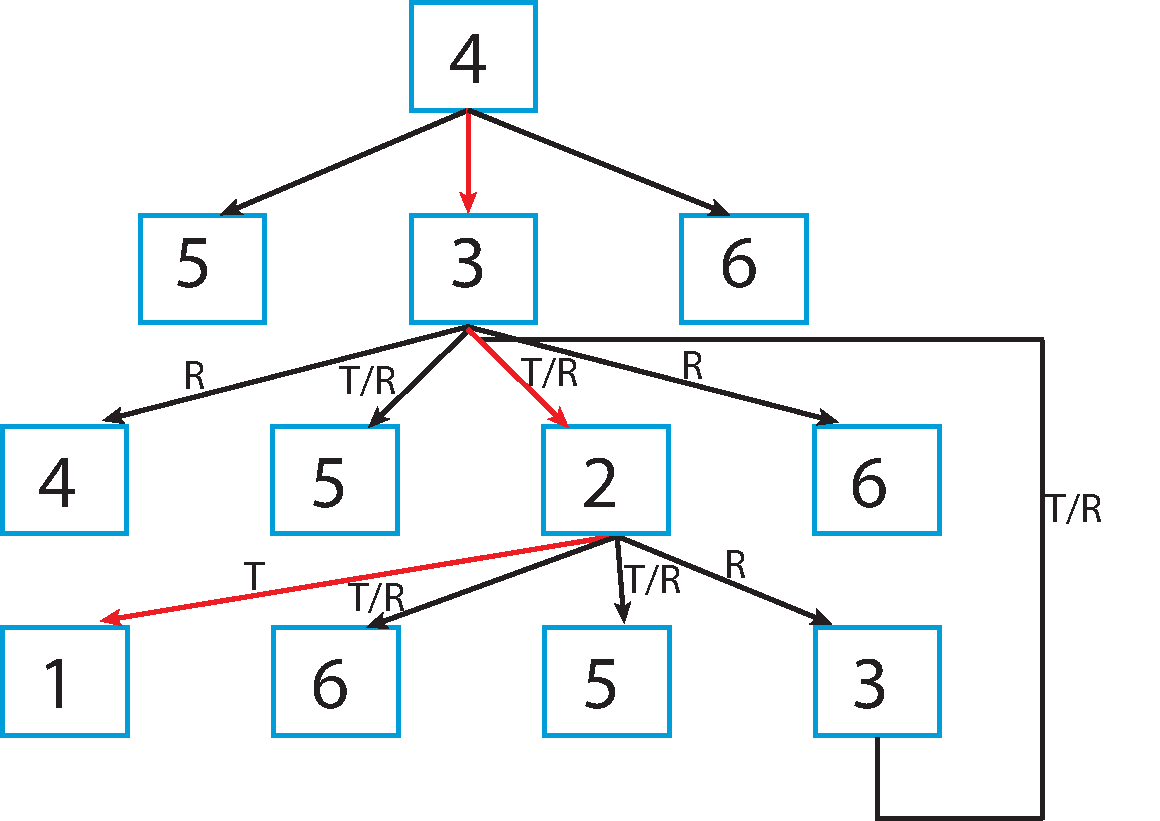
\includegraphics[width=0.6\textwidth]{tree_lens}
  \end{center}
  \caption{\textbf{Tree that show all the possible paths.} Considering Fresnel reflections the rays can reflect many times between line $2$ and $3$ before reaching either the target or one of the two detectors or the source again. At every reflection part of the energy of the ray is lost according to Fresnel reflections.}
\label{fig:tree_fresnel}
 \end{figure}
To find the boundary $\partial$\set{R}{}{}$(\Pi_1)$ of the region corresponding to that path $\Pi_1$ along a given a direction $\variabile{p} = \textrm{const}$, we start considering the rays with corresponding coordinates $(\variabile{q}^{\textrm{a}}, \variabile{p})$ and $(\variabile{q}^{\textrm{b}}, \variabile{p})$ located at the end points of the target PS, where $\variabile{q}^{\textrm{a}} = -\variabile{b}$ and $\variabile{q}^{\textrm{b}} = \variabile{b}$ and $\variabile{b}=5$. Then the bisection method and the inverse ray tracing is applied as explained in the previous chapter. We remark that in order to consider Fresnel effects, every time that the ray is traced back either the reflected or the refracted ray is considered according to the choice $C_1= (T,T)$. This allows us to determine the rays located on the boundaries $\partial$\set{R}{}{}$(\Pi_1)$. We indicate the coordinates of these rays with $(\variabile{q}^{\textrm{min}}(\Pi_1, \variabile{p}), \variabile{p})$ and $(\variabile{q}^{\textrm{max}}(\Pi_1, \variabile{p}), \variabile{p})$. \\ \indent
Since including Fresnel reflection the luminance at the target is not constant, an interpolation between the rays on the boundary $\partial$\set{R}{}{}$(\Pi_1)$ is needed. We indicate with $L_{\Pi_1}(\variabile{q},\variabile{p})$ the luminance corresponding to path $\Pi_1$. The interpolation between 
$(\variabile{q}^{\textrm{min}}(\Pi_1, \variabile{p}), \variabile{p})$ and $(\variabile{q}^{\textrm{max}}(\Pi_1, \variabile{p}), \variabile{p})$ allows us to calculate the profile of $L_{\Pi_1}(\variabile{q},\variabile{p})$ for every $\variabile{q}\in[\variabile{q}^{\textrm{min}}, \variabile{q}^{\textrm{max}}]$ and $\variabile{p}=\textrm{const}$.
% as it depends on the Fresnel coefficients which are related to the angle of the incident ray at every Fresnel line and to the index of refraction in which the ray travels (see Equations (\ref{eq:fresnel_pands2})). Therefore and interpolation between the coordinates of the rays on the boundaries gives the value of the luminance $L_{\Pi_1}(\variabile{q}, \variabile{p})$ along direction $\variabile{p}= \textrm{const}$ related to path $\Pi_1$.
Repeating the procedure for all the possible directions $\variabile{p}\in[-1,1]$, the profile of the partial luminance $L_{\Pi_1}$ given by all the rays that follow path $\Pi_1$ is computed for every $(\variabile{q}, \variabile{p})\in$\set{T}{}{}. 
\\ \indent Next another path $\Pi$ and the corresponding choice $C$ are considered. We remark that every path is associated to a unique choice but the vice versa is not always true. For example, the path $\Pi_2 = (1,2,3,2,3,4)$ considered in reverse order from the \point{T} to \point{S}, i.e. $\Pi_2^{\prime} = (4,3,2,3,2,1)$ can only be associate to the choice $C_2 = (T,R,R,T)$ which leads also to the inverse paths $\Pi_5^{\prime}= (4,3,2,3,2,5)$ and $\Pi_6^{\prime}= (4,3,2,3,2,6)$. The last two paths $\Pi_5^{\prime}$ and $\Pi_6^{\prime}$ are not paths from the target to the source, therefore they are not considered for the intensity calculation. Given a choice $C$ many paths are possible but only one is a physical path from the source to the target. Considering \textit{all} the possible choices, \textit{all} the physical paths are determined. The corresponding partial luminance $L_{\Pi}(\variabile{q}, \variabile{p})$ is calculated for every path $\Pi$.\\
\indent Finally, the total luminance $L(\variabile{q}, \variabile{p})$ is given by:
\begin{equation}\label{eq:luminance_fresnel}
L(\variabile{q}, \variabile{p}) = \sum_{\Pi}L_{\Pi}(\variabile{q}, \variabile{p}),
\end{equation} 
where the summation is over all the possible paths. 
From an integration of $L(\variabile{q}, \variabile{p})$ the intensity at the target is given by:
\begin{equation}\label{eq:intensity_fresnel}
I(\variabile{q}, \variabile{p}) = \int_{\mbox{\set{Q}{}{}}}L(\variabile{q}, \variabile{p})\textrm{d}\variabile{q}.
\end{equation}
\\ \indent In the next section numerical results are shown.
\section{Numerical results}
In this section the numerical results for the lens are presented. We detect the boundaries of the regions formed by the rays that follow the path for every physical path, that is a path from the source to the target. To this purpose we decide a priori the choice that has to be done at every intersection of the ray with a Fresnel lens. The choice establishes whether the reflected or the transmitted part of the incident ray has to be considered when the rays traced back hit a Fresnel line.\\ \indent
We start considering the choice $C_1 = (T,T)$. Note that this choice correspond to the physical path $\Pi_1=(1,2,3,4)$.
Indeed, every ray traced back hit the right curved line (line $3$) and is split in two rays, at this point the reflectance $\mathcal{R}$ and transmittance $\mathcal{T}$ are calculated and, according to the first component of $C_1$, the transmitted ray is considered and traced back further with the corresponding power $\mathcal{T}$. This ray continues to propagate through the system until it hits either the detectors (line $5$ and $6$) or the curved line $2$.
In case it hit the detectors the procedure is stopped, otherwise the ray is split again into two more rays. Again, according to the second component of $C_1$, the transmitted ray is considered and it continues its trajectory reaching either the detectors or the source (line $1$). 
In Figure \ref{fig:ray_path1} we draw in red and example of ray that follows path $\Pi_1 = (1,2,3,4)$.\\ \indent 
Using the inverse numerical ray mapping and taking into account the choice $C_1$ every time that the inverse ray tracing is applied and the rays hit a Fresnel line, the boundaries $\partial$\set{R}{}{}$(\Pi_1)$ are found. In Figure \ref{fig:boundary_path1} $\partial$\set{R}{}{}$(\Pi_1)$ is shown in blue. To verify whether this boundary is correct we trace around $10^4$ rays using forward QMC ray tracing imposing that at every interaction of the ray with lines $2$ and $3$ always the transmitted part of is considered. These rays are traced in red in Figure \ref{fig:boundary_path1}. The picture shows that all the rays traced are inside the boundary $\partial$\set{R}{}{}$(\Pi_1)$ which is, therefore, calculated correctly.
\begin{figure}[t]
\centering
\begin{subfigure}[t]{.45\textwidth}
  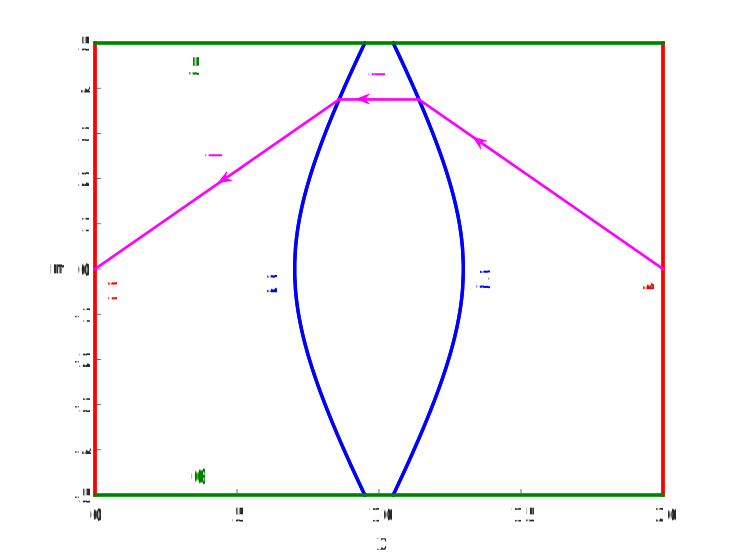
\includegraphics[width=\textwidth]{lens_path1}
 \caption{\textbf{Ray traced back from the target to the source}. The rays follows path $\Pi_1 = (1,2,3,4)$ corresponding to the choice $C_1=(T,T)$ from the target to the source. The percentage of power of the ray at the source is }
  \label{fig:ray_path1}
\end{subfigure}%
\hfill
\begin{subfigure}[t]{.45\textwidth}
  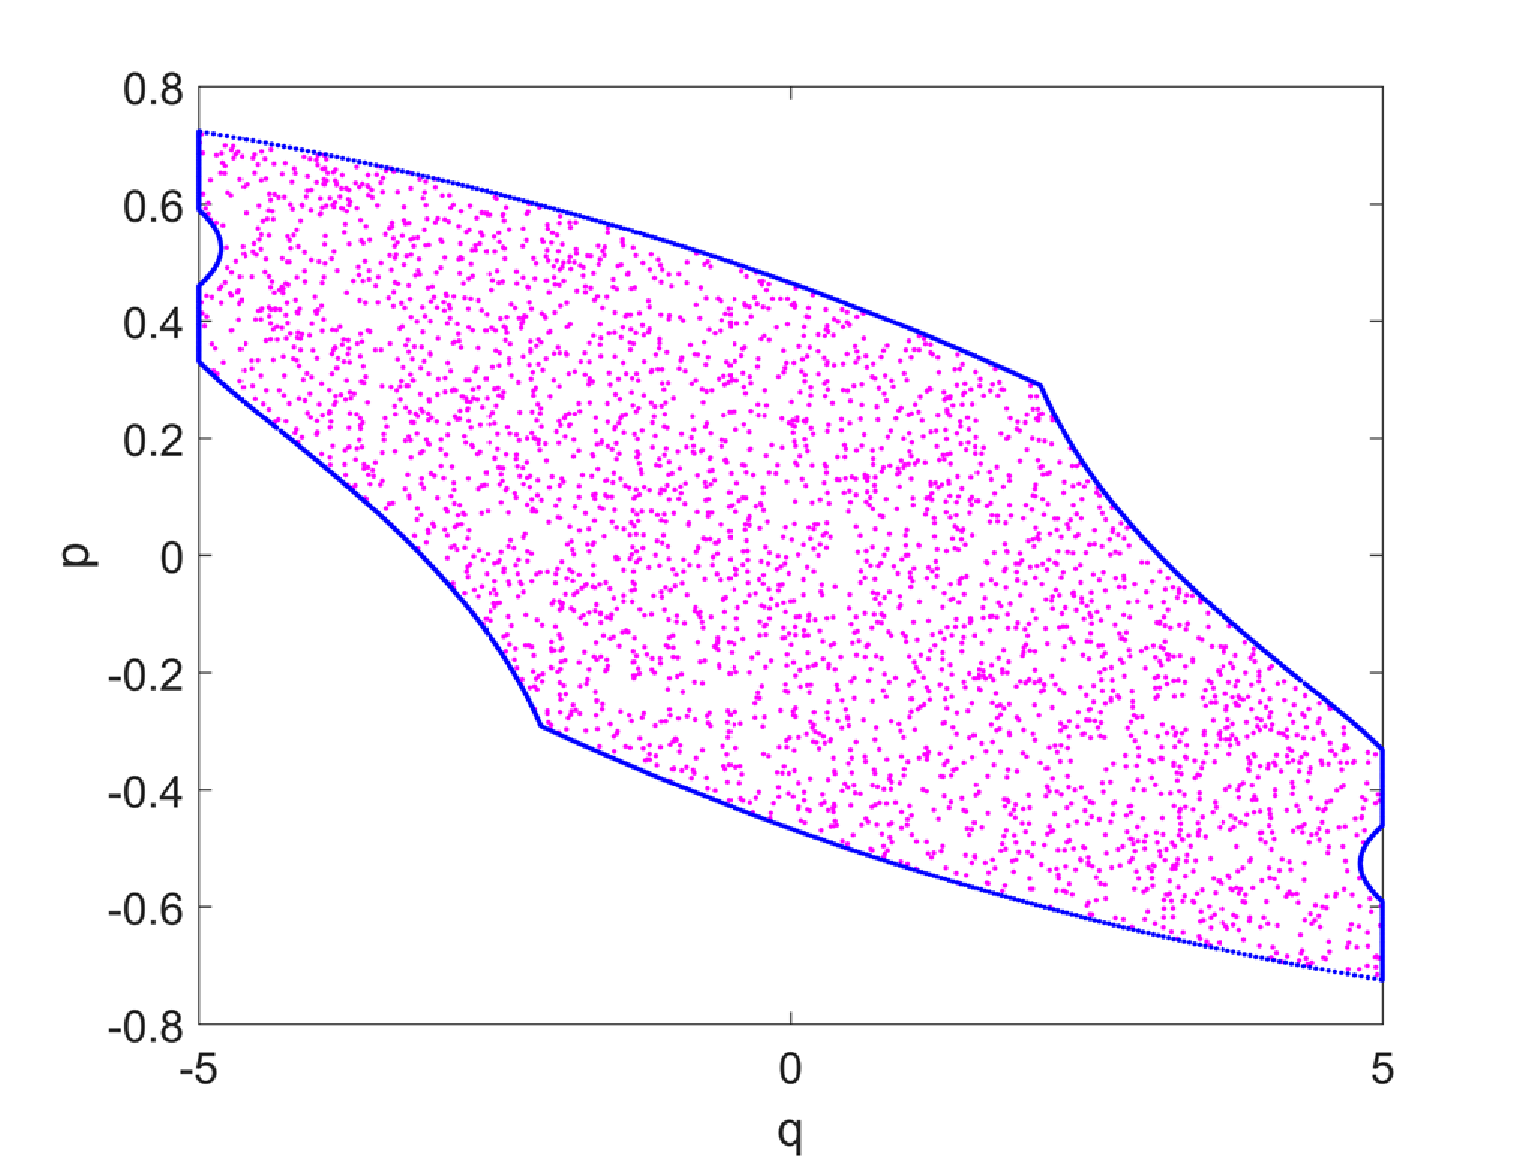
\includegraphics[width=\textwidth]{path_lens1}
  \caption{\textbf{Boundary $\partial$\set{R}{}{}$(\Pi_1)$.} The boundary is depicted with the blue line, the red rays are traced using QMC ray tracing and considering always the transmitted ray.} %
  \label{fig:boundary_path1}
\end{subfigure} %
\caption{\textbf{Computation of the boundary $\partial$\set{R}{}{}$(\Pi_1)$.}}
\end{figure}
\\ \indent To detect the other paths we need to consider all the possible choice. We continue considering the choice $C_2 = (T, R, R, T)$,. This means that once the ray is traced back from the target, if it hits the line $3$, the transmitted part is considered according to the first component of $C_2$ and it is traced back further with its corresponding power given by $\mathcal{T}$. If the transmitted ray does not hit the detectors, it hits line $2$ where it is split again. Now the reflected part of the ray is considered according to the second component of $C_2$. The power of the reflected ray is given by the reflectance $\mathcal{R}$ multiplied by the power of the incident ray. The rays continues to propagates inside the system, if it hits line $3$ it is reflected according to the third component of $C_2$ and, in case it hit line $2$ next, it is finally transmitted according to the last component of $C_2$. If the ray reach finally the source, it follows the physical path $\Pi_2 = (1,2,3,2,3,4)$. 
In Figure \ref{fig:ray_path2} we show in green a ray traced back from the target to the source that follows path $\Pi_2$. The numerical inverse ray mapping applied considering the choice $C_2$ every time that the inverse ray tracing is employed, provides the boundary of the region $\partial$\set{R}{}{}$(\Pi_2)$ which is depicted in blue in Figure \ref{fig:boundary_path2}. To properly detect the boundary we divided the target PS into $\textrm{Ni}=10$ bins as explained in Section \ref{}. Likewise for the boundary $\partial$\set{R}{}{}$(\Pi_1)$, to prove that the method computes the boundary correctly we traced $10^4$ rays using QMC ray tracing and and using the decision $C_2$ at every intersection with line $2$ and $3$. These rays are traced in green in Figure \ref{fig:boundary_path2}. We observe that all the rays traced are located inside the blue line, therefore the boundary $\partial$\set{R}{}{}$(\Pi_2)$ is calculated correctly.
\begin{figure}[t]
\centering
\begin{subfigure}[t]{.45\textwidth}
  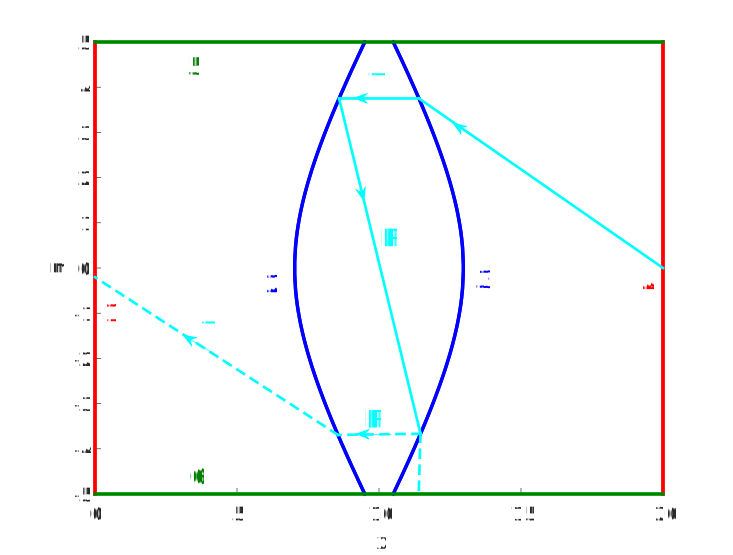
\includegraphics[width=\textwidth]{lens_path2}
 \caption{\textbf{Ray traced back from the target to the source}. The rays follows path $\Pi_2 = (1,2,3,2,3,4)$ corresponding to the choice $C_2=(T,R,R,T)$ from the target to the source. The percentage of power of the ray at the source is }
  \label{fig:ray_path2}
\end{subfigure}%
\hfill
\begin{subfigure}[t]{.45\textwidth}
  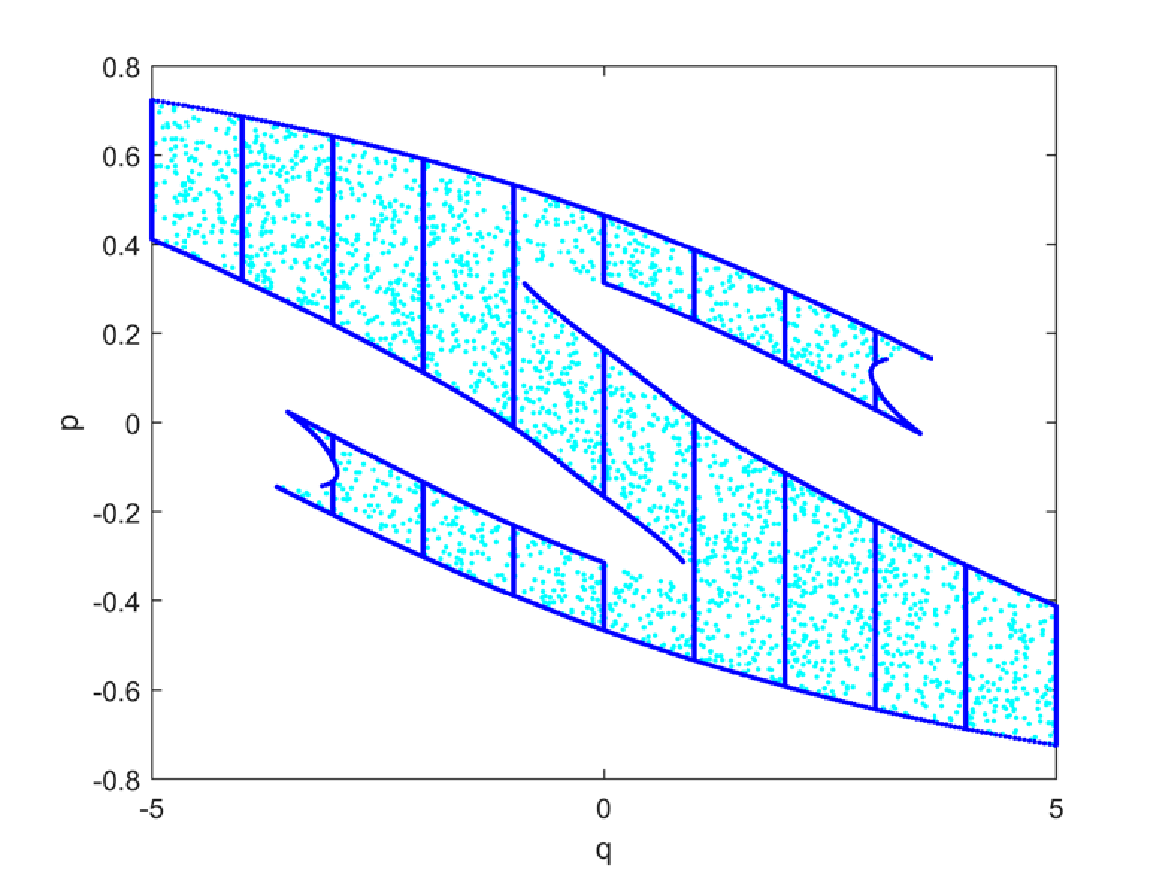
\includegraphics[width=\textwidth]{path_lens2}
  \caption{\textbf{Boundary $\partial$\set{R}{}{}$(\Pi_2)$.} The boundary is depicted with the blue line, the green rays are traced using QMC ray tracing with $10^4$ and considering two reflections between the lenses.} %
  \label{fig:boundary_path2}
\end{subfigure} %
\caption{\textbf{Computation of the boundary $\partial$\set{R}{}{}$(\Pi_2)$.}}
\end{figure}
\\ \indent Note that more than two reflection can occur between line $2$ and $3$, thus the procedure continues considering the choice $C_3 = (T,R,R,R,R,T)$ that leads to four reflections between line $2$ and $3$. Every ray traced back from the source is first transmitted, then reflected between $2$ and $3$ four times and finally transmitted again. If the ray hits the source then it follows the physical path $\Pi_{3} = (1,2,3,2,3,2,3,4)$ corresponding to the choice $C_3$ is found. A ray that follow path $\Pi_3$ is depicted in black in Figure \ref{fig:ray_path3}. The inverse ray mapping with the choice $C_3$ gives the boundary $\partial$\set{R}{}{}$(\Pi_3)$ depicted in blue in Figure \ref{fig:boundary_path3}. This boundaries is obtained dividing the target PS into $\textrm{Ni}=10$ bins and applying the inverse ray mapping to each bin. The black dots correspond to the rays in target PS obtained using QMC ray tracing with $10^4$ rays where at every intersection with the Fresnel lines either the reflected or the transmitted ray are selected according to choice $C_3$. Also in this case we found that the boundary computation is correct.
\begin{figure}[t]
\centering
\begin{subfigure}[t]{.45\textwidth}
  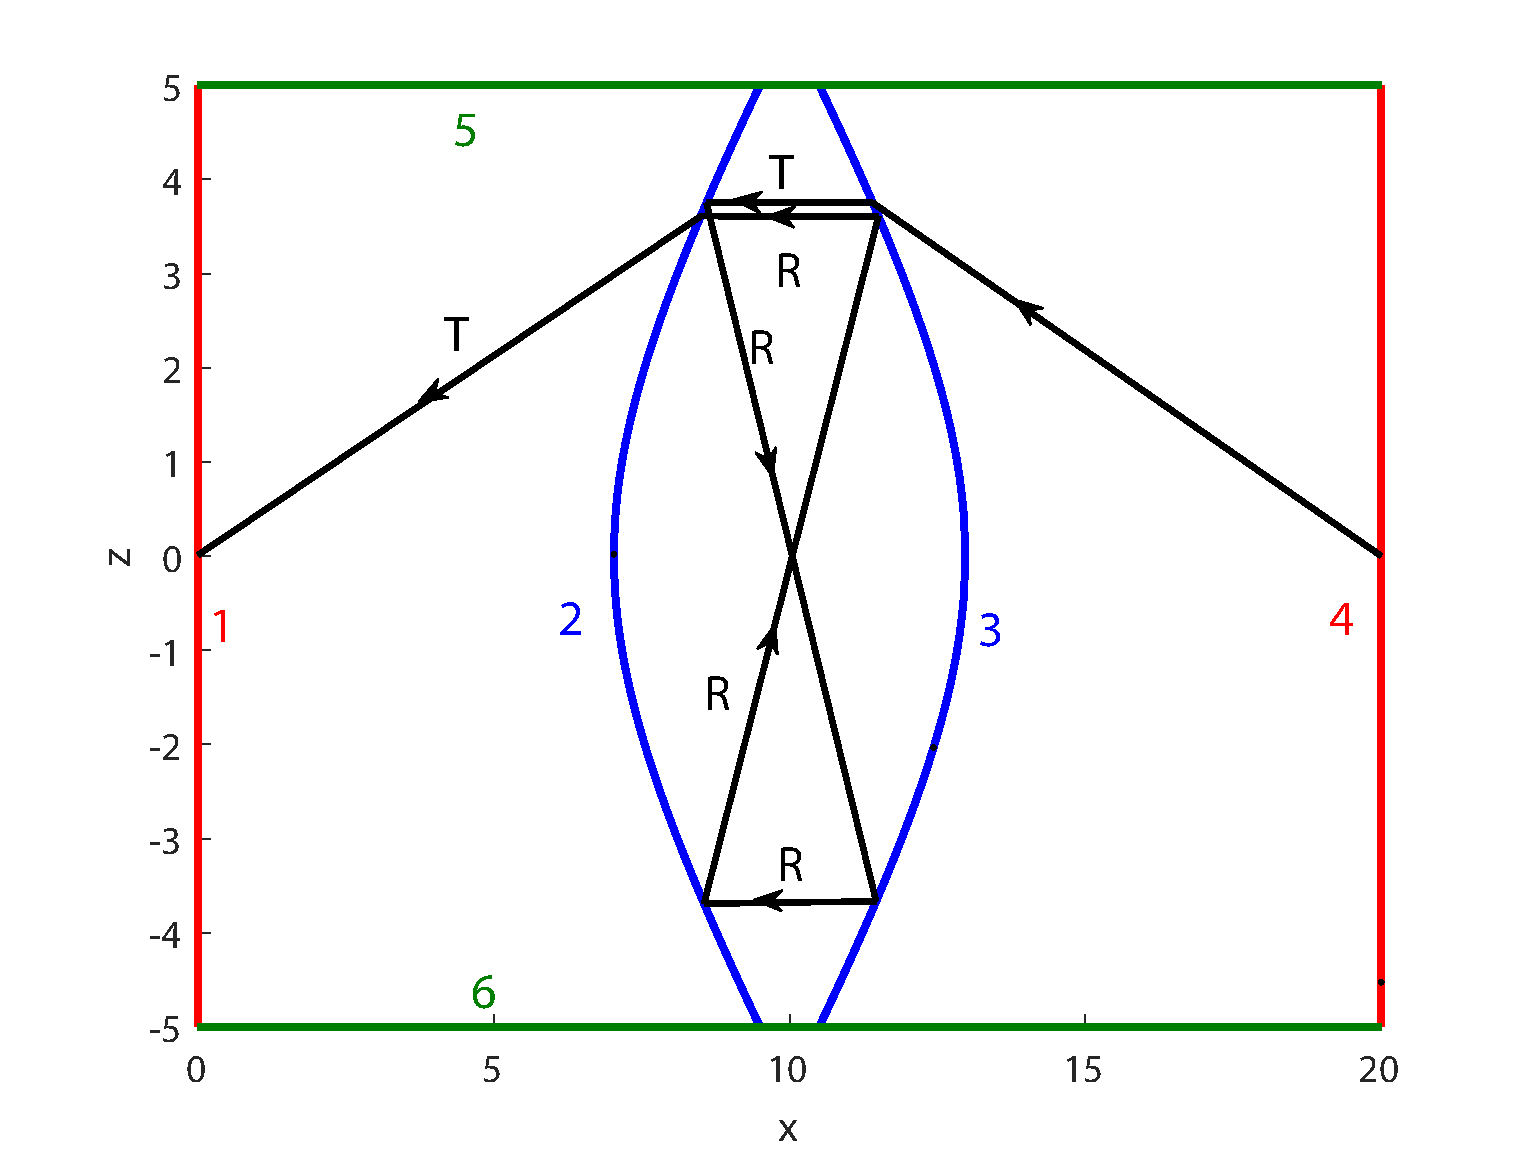
\includegraphics[width=\textwidth]{lens_path3}
 \caption{\textbf{Ray traced back from the target to the source}. The rays follows path $\Pi_3 = (1,2,3,2,3,2,3,4)$ corresponding to the choice $C_3=(T,R,R,R,R,T)$ from the target to the source. The percentage of power of the ray at the source is}
  \label{fig:ray_path3}
\end{subfigure}%
\hfill
\begin{subfigure}[t]{.45\textwidth}
  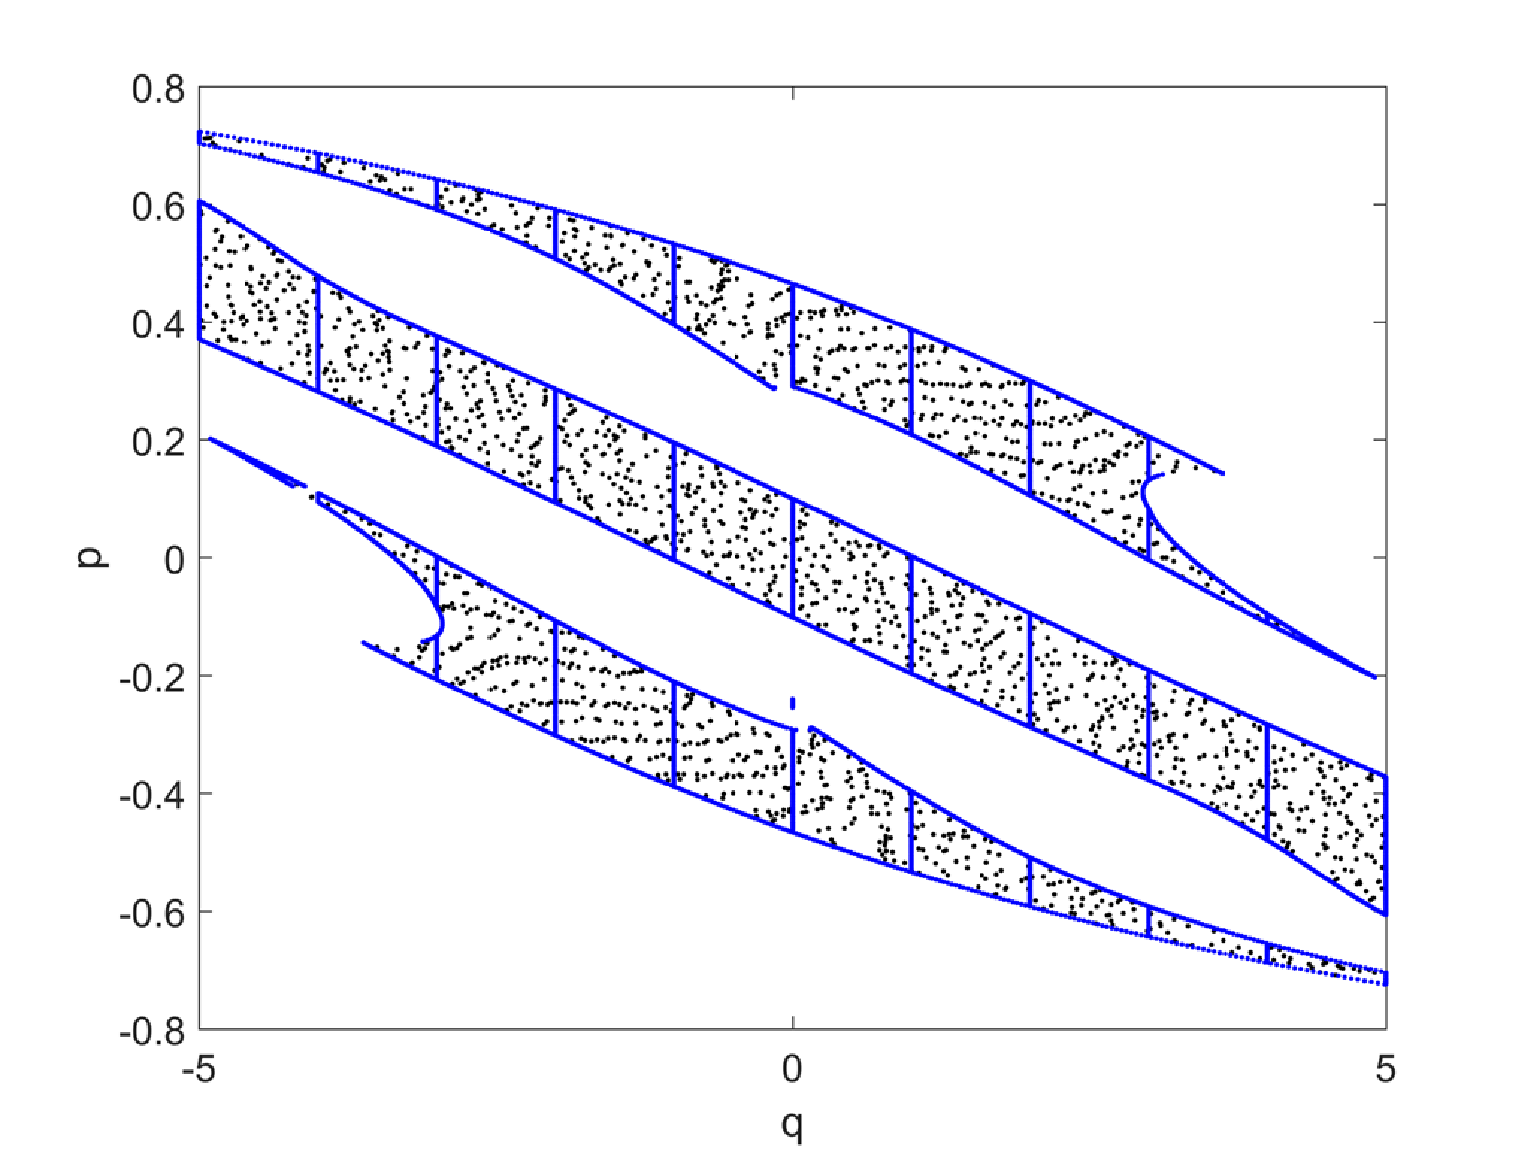
\includegraphics[width=\textwidth]{path3_fresnel}
  \caption{\textbf{Boundary $\partial$\set{R}{}{}$(\Pi_3)$.} The boundary is depicted with the blue line, the black rays are traced using QMC ray tracing with $10^4$ and considering four reflections between the lenses.} %
  \label{fig:boundary_path3}
\end{subfigure} %
\caption{\textbf{Computation of the boundary $\partial$\set{R}{}{}$(\Pi_3)$.}}
\end{figure}
\\ \indent Since rays with multiple reflections do not bring a significant amount of power, we decide do not to consider the rays with more than four reflections as they do not give a significant contribution to the output photometric variables. However, the inverse ray mapping is able to detect \textit{all} the boundaries of the regions with positive luminance in target PS. The procedure can be stopped accordingly to the desired accuracy. The more reflections are considered, the better accuracy is obtained. \\ \indent
We remark now that the luminance at the target cannot be constant because every ray has a certain amount of energy that depends on the Fresnel coefficients. Because of this, an interpolation between the rays on the boundaries is needed to compute the profile of the luminance at the target. In Figure \ref{fig:interpolation1} we show the procedure to compute the luminance related to path $\Pi_1$ along direction $\variabile{p}=0$. The rays corresponding to the coordinates $(\variabile{q}(\Pi_1, \variabile{p}), \variabile{p})$ with $\variabile{q}\in[\variabile{q}^{\textrm{min}}(\Pi_1,\variabile{p}), \variabile{q}^{\textrm{max}}(\Pi_1,\variabile{p})]$ and $\variabile{p}=0$ are traced from the source to the target using the inverse ray tracing and taking into account of the choice $C_1$ at every intersection with the Fresnel lines. The rays traced are depicted in red. The luminance $L_{\Pi_1}(\variabile{q}, \variabile{p})$ is calculated for every $\variabile{q}\in[\variabile{q}^{\textrm{min}}(\Pi_1,\variabile{p}), \variabile{q}^{\textrm{max}}(\Pi_1,\variabile{p})]$ and $\variabile{p}=0$. Its profile is depicted in Figure \ref{fig:luminance_fresnel}.
\begin{figure}[t]
\centering
\begin{subfigure}{.45\textwidth}
  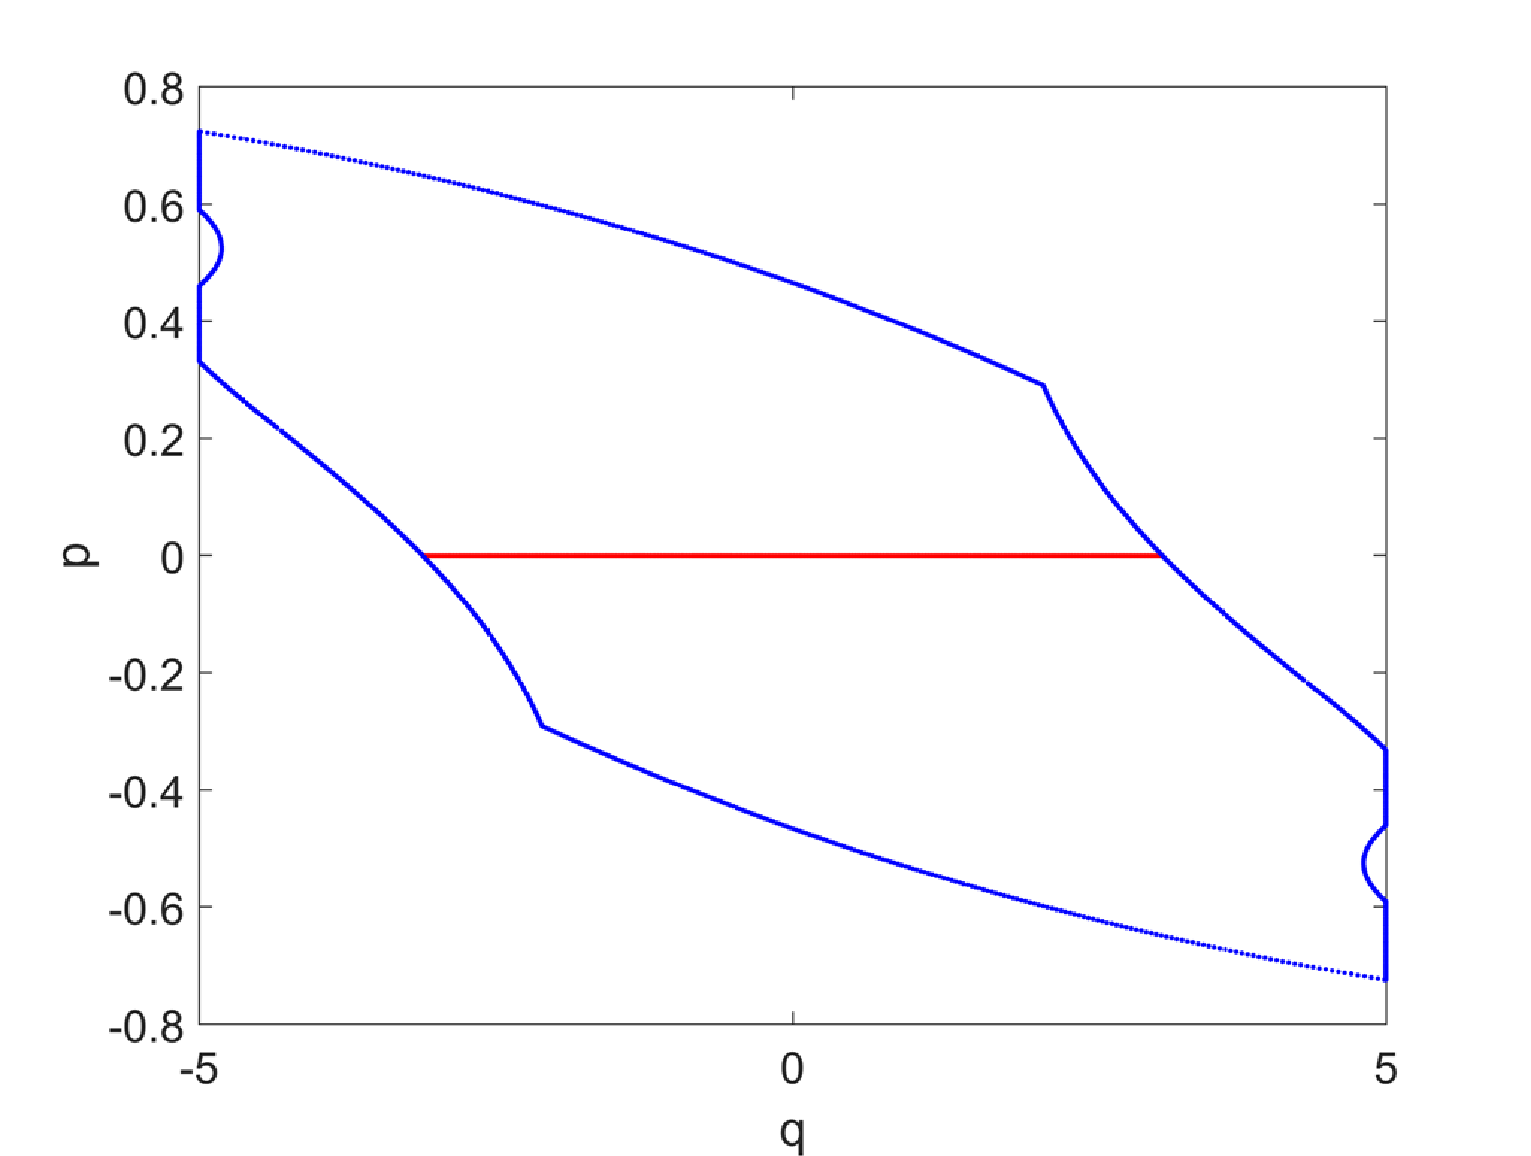
\includegraphics[width=\textwidth]{interpolation1}
 \caption{Interpolation between the rays on $\partial$\set{R}{}{}$(\Pi_1)$ along direction $\variabile{p}=0$.}
  \label{fig:interpolation1}
\end{subfigure}%
\hfill
\begin{subfigure}{.45\textwidth}
  \includegraphics[width=\textwidth]{luminance}
  \caption{Luminance $L_{\Pi_1}(\variabile{q}, 0)$ related to path $\Pi_1$ along direction $\variabile{p}=0$ and with $\variabile{q}\in[\variabile{q}^{\textrm{min}}(\Pi_1, \variabile{p}), \variabile{q}^{\textrm{max}}(\Pi_1, \variabile{p})]$.} %
  \label{fig:luminance_fresnel}
\end{subfigure} %
\caption{\textbf{Determination of the partial luminance.} $L_{\Pi_1}(\variabile{q}, 0)$ is related to path $\Pi_1$ along direction $\variabile{p}=0$.} 
\end{figure}
\\\indent 
Repeating the interpolation along all the possible directions $\variabile{p}\in[-1,1]$, the luminance $L_{\Pi_1}(\variabile{q}, \variabile{p})$ related to the rays that follow path $\Pi_1$ is found for every $\variabile{p}\in[-1,1]$ and $\variabile{q}\in[\variabile{q}^{\textrm{min}}(\Pi_1,\variabile{p}), \variabile{q}^{\textrm{max}}(\Pi_1,\variabile{p})]$. The same procedure is applied to all the paths considered and the luminance corresponding to each path is calculated. The total luminance $L(\variabile{q}, \variabile{p})$ is given by the sum in Equation (\ref{eq:luminance_fresnel}). Finally, the intensity is computed using Equation (\ref{eq:intensity_fresnel}). \\ \indent
In this thesis we do not show the numerical results of the total luminance and intensity because there is still some work in progress. To validate the method we need to calculate the luminance along every possible direction and compare it with a reference luminance obtained for example using either MC or QMC ray tracing. Our expectation is that the inverse ray mapping is suitable also for systems with Fresnel reflection. Indeed, our first results show that the boundaries of the regions with positive luminance are calculated correctly. Once the boundaries are found also the luminance and the intensity can be computed applying an interpolation between the rays on the boundaries along every possible direction. Furthermore we expect that the method is much more accurate and faster than both MC and QMC ray tracing. This is due to the fact that we can analyse every single path independently from the others.  
\section{Conclusion and outlook}